\documentclass[a4paper, 11pt,reqno]{article}
\input{/Users/olivierglorieux/Desktop/BCPST/2020:2021/preambule.tex}
\newif\ifshow
\showtrue
\input{/Users/olivierglorieux/Desktop/BCPST/2021:2022/ifshow.tex}

\geometry{hmargin=1.0cm, vmargin=1.5cm}


\author{Olivier Glorieux}


\begin{document}

\title{DM vacances février  
}
\begin{exercice}
Revoir les régles de calculs sur $\exp$  et $\ln$ 
\footnote{($\exp(a+b)= \exp(a)\exp(b)$, $\ln(ab)=\ln(a)+\ln(b)$...) } et leurs graphes et leurs limites...
\end{exercice}
\begin{correction}
A vous de travailler ! 
\end{correction}


\begin{exercice}
Calculer les limites suivantes 
\begin{enumerate}
\item $\lim_{x\tv 1} \frac{x-1}{\cos(\frac{\pi x}{2})}$
\item $\lim_{x\tv 0} \frac{x\ln(x)}{e^x-1}$
\item $\lim_{x\tv +\infty} \frac{\ln(x^2)}{\ln(x+1)}$
\item $\lim_{x\tv +\infty} \frac{\ln(x) e^{x^2}}{x^x}$
\end{enumerate}
\end{exercice}


\begin{correction}
\begin{enumerate}
\item  ( FI $\frac{0}{0}$ - pas nécessaire sur une copie) 
On fait un changement de variable : $y=x-1$.
$$\frac{x-1}{\cos(\frac{\pi x}{2})} = \frac{y}{\cos(\frac{\pi y}{2}+\frac{\pi}{2})}=-\frac{y}{\sin(\frac{\pi y}{2})}$$
Or $\sin(u)\equivalent{0} u$ et $\ddp \lim_{y \tv 0} \frac{\pi y}{2} =0$ donc,  $\sin(\frac{\pi y}{2})\equivalent{0} \frac{\pi y}{2}$. Ainsi 
$$\lim_{x\tv 1} \frac{x-1}{\cos(\frac{\pi x}{2})} = \lim_{y\tv 0} -\frac{y}{\sin(\frac{\pi y}{2})}= -\frac{2}{\pi}.$$
\item  ( FI $\frac{0}{0}$ - pas nécessaire sur une copie) 
D'après le cours $e^x-1\equivalent{0}x$ donc $ \frac{x\ln(x)}{e^x-1} \equivalent{0} \ln(x)$
Ainsi : $$\lim_{x\tv 0} \frac{x\ln(x)}{e^x-1}=-\infty.$$
\item  ( FI $\frac{+\infty}{+\infty}$ - pas nécessaire sur une copie) 
$\ln(x^2)= 2\ln(x)$ et  $\ln(x+1) = \ln(x) + \ln\left( 1+\frac{1}{x}\right)\equivalent{+\infty }\ln(x)$. Donc 
$$\lim_{x\tv +\infty} \frac{\ln(x^2)}{\ln(x+1)}=2$$
\item  ( FI $\frac{+\infty}{+\infty}$ - pas nécessaire sur une copie) 
La puissance est une fonction de la variable $x$, on passe donc à la forme exponentielle : $x^x =\exp(x\ln(x))$.
\begin{align*}
\frac{\ln(x) e^{x^2}}{x^x }&= \frac{\ln(x) \exp(x^2)}{exp(x\ln(x)} \\
&= \ln(x) \exp(x^2-x\ln(x))\\ 
&=\ln(x) \exp(x(x-\ln(x))
\end{align*}
Or $x-\ln(x) \tv_{+\infty} +\infty$ par croissance comparée. Donc $\exp(x(x-\ln(x))\tv_{+\infty} +\infty$  et finalement 
$$\lim_{x\tv +\infty} \frac{\ln(x) e^{x^2}}{x^x} =+\infty.$$

\end{enumerate}

\end{correction}






\begin{exercice}
Donner des équivalents simples de 
\begin{enumerate}
\item Quand $x\tv 1$ de $\frac{\ln(x)}{\sqrt{x^2-1}} $
\item Quand  $x\tv 0$ de $\frac{x\ln(x)}{e^x-1}$
\item Quand  $n\tv +\infty$  de $\ddp \sum_{k=0}^{2n}( k^2+k ) $
\end{enumerate}
\end{exercice}


\begin{correction}
\begin{enumerate}
\item 
On fait un changement de variable $y=x-1$, on obtient 
$$\frac{\ln(x)}{\sqrt{x^2-1}} = \frac{\ln(y+1)}{\sqrt{y^2+2y}} $$
Or $\ln(y+1)\equivalent{0} y$ et $\sqrt{y^2+2y}= \sqrt{y(y+2)}\equivalent{0}\sqrt{2}\sqrt{y}$
Donc $$\frac{\ln(y+1)}{\sqrt{y^2+2y}} \equivalent{0}\frac{y}{\sqrt{2}\sqrt{y}} \equivalent{0}\frac{\sqrt{y}}{\sqrt{2}}.$$
On revient à la variable $x$ : 

$$\frac{\ln(x)}{\sqrt{x^2-1}} \equivalent{1} \frac{\sqrt{x-1}}{\sqrt{2}}$$

\item On a déjà vu cette expression à l'exercice précédent : on obtient 
$$\frac{x\ln(x)}{e^x-1}\equivalent{0} \ln(x).$$
\item  
\begin{align*}
\sum_{k=0}^{2n} k^2+k   &=\sum_{k=0}^{2n} k^2 +\sum_{k=0}^{2n} k  \\
										&= \frac{2n(2n+1)(2(2n)+1)}{6}  + \frac{2n(2n+1)}{2}\\
										&=\frac{16n^3 +R(n)}{6} + \frac{4n^2+2n}{2}
\end{align*}
où $R$ est un polynôme (que je n'ai pas envie de calculer) de degré inférieur strictement à $3$. 
Or en $ +\infty $  une fonction polynomiale est équivalent à son terme de plus haut degré, on a donc : 
$$\frac{16n^3 +R(n)}{6} + \frac{4n^2+2n}{2}\equivalent{+\infty} \frac{16n^3}{6}$$
D'où
$$\sum_{k=0}^{2n} k^2+k  \equivalent{+\infty} \frac{8n^3}{3}$$


\end{enumerate}
\end{correction}





\begin{exercice} 
Soit $\suite{u}$ la suite définie par 
$$\left\{ 
\begin{array}{ccl}
u_0&=&2\\
u_{n+1} &=&1 +\frac{1}{u_n}
\end{array}
\right.$$

\begin{enumerate}
\item Calculer $u_1$.
\item Etudiez la fonction $f: x\mapsto 1+\frac{1}{x}$. (Domaine de définition, limites et variations) 
%\item Montrer  que pour tout $n\in \N$, $1\leq u_n\leq 2$.
\item Résoudre $f(x)=x$. On note $\alpha$ l'unique solution dans $\R^*_+$. 
\item Montrer que $u_1<\alpha <2$.
\item On note $I=[1,\alpha]$ et $J=[\alpha,2]$. Montrer que $f(I)\subset J$ et $f(J)\subset I$.
\item On considère les suites $\suite{a}$ et  $\suite{b}$ définies par 
$$a_n=u_{2n} \quad b_n =u_{2n+1}.$$
Enfin on note $A$ la fonction définie pour tout $x$ par $A(x)=f\circ f(x)$.
 Montrer que $a_{n+1} =A (a_n)$. On peut montrer de manière similaire que 
 $b_{n+1} =A(b_n) $, on ne demande pas de le prouver. 
 \item Soit $F$ une fonction réelle. Soient $\cE $ et $\cF$ deux sous-ensembles de $\R$. Montrer que si $\cE\subset \cF$ alors $F(\cE)\subset F(\cF)$. En déduire que  $I$ est stable par $A$. De même, on pourrait montrer que $J$ est stable par $A$, on ne demande pas de le prouver. 
\item Montrer que pour tout $x\in D_f$, $A(x)-x =\frac{-x^2+x+1}{x+1}$ 
\item Résoudre $A(x)\geq x$ sur $]0,+\infty[$. 
\item  En déduire que $\suite{a}$ est décroissante et $\suite{b}$ est croissante. 
\item Montrer que $\suite{a}$ et $\suite{b}$ convergent, calculer leur limite. 
\item En déduire que $\suite{u}$ converge et calculer sa limite. 
\item \begin{enumerate}
\item Ecrire une fonction Python \texttt{u} qui prend en paramètre un entier $n$ et qui renvoie la valeur de $u_n$
\item Ecrire une fonction Python \texttt{limiteu} qui prend en paramètre un reel $\epsilon>0$ et  qui renvoie la valeur de du premier rang $n_0\geq 0$ tel que $|u_{n_0} -\ell|\leq \epsilon$ 
\end{enumerate}

\end{enumerate}

\end{exercice}

\begin{correction}
\begin{enumerate}
\item $u_1=\frac{3}{2}$
\item L'ensemble de définition est $\R^*$.  $f$ est dérivable sur son ensemble de définition et 
$$f'(x) =\frac{-1}{x^2}$$
On obtient le tableau de variation suivant 



\begin{tikzpicture}
   \tkzTabInit{$x$ / 1 , $f(x)$ / 2}{$-\infty$, 0, $+\infty$}
   \tkzTabVar{+/ $1$,  -D+/ $-\infty$ /$+\infty$,  -/ $1$}
\end{tikzpicture}

\item $\frac{1}{x}+1=x\equivaut x^2-1-x=0$
Dont les solutions sont $\{ \frac{1\pm\sqrt{5}}{2}\}$. L'unique solution dans $\R^+$ est $\alpha = \frac{1+\sqrt{5}}{2}$

\item $\frac{1+\sqrt{5}}{2}\leq 2 \equivaut \sqrt{5}\leq 3 \equivaut 5\leq 9$ qui est vrai. 

$u_1 \leq \frac{1+\sqrt{5}}{2} \equivaut 2\leq \sqrt{5} \equivaut 4 \leq 5$ qui est vrai. 

\item $f(\alpha) =\alpha$, $f(2) =\frac{3}{2}$. comme $f$ est décroissante sur $J$ on a bien pour tout $x\in J$ 
$f(2)\leq f(x)\leq f(\alpha)$. Donc 
$$\frac{3}{2}\leq f(x) \leq \alpha.$$ 
Comme $1\leq \frac{3}{2}$ on  a bient $f(J)\subset I$. 

Un argument similaire montre que pour tout $x\in I$ on  a:
$$\alpha =f(\alpha) \leq f(x)\leq f(1)=2$$
et ainsi $f(I)\subset J$. 
\item $\forall n\in\N$:
$$A(a_n) = f\circ f(a_n)=f\circ f (u_{2n})= f(u_{2n+1}) = u_{2n+2}=a_{n+1}$$

\item On suppose donc que $\cE\subset \cF$. Soit $y\in F(\cE)$ c'est à dire qu'il existe $x\in \cE$ tel que $f(x)=y$
Comme $\cE\subset \cF$,on a $x\in \cF$, donc $y=f(x)\in \cF$. Ainsi en tuilisant la question 5 on obtient : 
$$f\circ f(I) \subset f(J) \subset I$$

\item $A(x)=f(f(x))=f(  1+\frac{1}{x}) =1 + \frac{1}{1+\frac{1}{x}}= \frac{2x+1}{x+1} $
Donc $A(x) - x = \frac{2x+1}{x+1}  -x = \frac{2x+1-x^2 -x}{x+1} = \frac{-x^2+x+1}{x+1}$ 
\item $A(x)-x\geq 0 \equivaut \frac{-x^2+x+1}{x+1}$ dont les solutions sur $\R_+^*$ sont $S= ]0,\alpha [$. 
\item $a_0 =u_0 \in J$, comme $J$ est stable par $A$ on déduit par récurrrence que $\forall n\in \N,\, $ $a_n\in J$.
De même comme $u_1=v_1 \in I$, et $I$  est stable par $A$ on déduit que $\forall n\in \N,\,$ $b_n\in I$.
Pour tout $n\in \N$ on  a 
$$a_{n+1}-a_n= A(a_n)-a_n$$
Comme $ A(x)-x\leq 0 $ sur $J$ et $a_n\in J$, on a bien $a_{n+1}-a_{n}\leq 0$ donc $\suite{a}$ est décroissante. 

De même, pour tout $n\in \N$ on  a 
$$b_{n+1}-b_n= A(b_n)-b_n$$
Comme $ A(x)-x\geq 0 $ sur $I$ et $b_n\in I$, on a bien $b_{n+1}-b_{n}\geq 0$ donc $\suite{b}$ est croissante. 


\item Les suites $\suite{a}$ et $\suite{b}$ sont monotones et bornées. Elles sont donc convergentes d'après le théorème de la limite monotone. Notons $\ell_a$ la limite de $\suite{a}$ et $\ell_b$ la limite de $\suite{b}$ (Nous n'avons pas montré que ces suites étaient adjacentes, nous ne pouvons pas directement dire que les limites sont identiques) 

Par unicité de la limite $\lim_{n\tv infty } a_{n+1}=\ell_a$. Comme $A$ est continue sur $\R_+$ on a $\lim_{n\tv \infty} A(a_n)  = A(\ell_a)$. Ainsi $\ell_a$ vérifie $A(\ell_a) = \ell_a$. on a vu à la quetsion  9 que cette avait pour unique solution $\ell_a=\alpha= \frac{1+\sqrt{5}}{2}$. Le même argument montre que $\ell_b =\alpha$. 

\item Les deux suites extraites $u_{2n}$ et $u_{2n+1}$ convergent et ont même limite. La suite $\suite{u}$ est donc aussi convergente et a pour limite $\alpha$. 


\item 
\begin{lstlisting}
from math import *
def u(n):
  x=0
  for i in range(n):
    x=1+1/x
   return(x)

def limiteu(epsilon):
  n=0
  l=(1+sqrt(5))/2
  while abs(u(n)-l)>epsilon:
    n=n+1
  return(n)
  
def limiteu2(epsilon): #autre solution
  n=0
  l=(1+sqrt(5))/2
  u=2
  while abs(u-l)>epsilon:
    n=n+1
    u=u+1/u
  return(n)
  

def limiteab(epsilon):
  n=0
  while abs(u(2*n)-u(2*n+1))>epsilon:
    n=n+1
  return(n)
\end{lstlisting}

\end{enumerate}
\end{correction}






\end{document}